 \documentclass[xcolor=dvipsnames,table]{beamer}

\usepackage{latexsym}
\usepackage[utf8]{inputenc}
\usepackage[brazil]{babel}
\usepackage{amssymb}
\usepackage{amsmath}
\usepackage{stmaryrd}
\usepackage{fancybox}
\usepackage{datetime}
\usepackage[T1]{fontenc}
\usepackage{graphicx}
\usepackage{graphics}
\usepackage{url}
\usepackage{algorithmic}
\usepackage{algorithm}
\usepackage{acronym}
\usepackage{array}
\usepackage{tikz}

\usepackage{enumitem}

\newtheorem{definicao}{Definio}
\newcommand{\tab}{\hspace*{2em}}

\mode<presentation>
{
  \definecolor{colortexto}{RGB}{0,0,0}
 
  \setbeamertemplate{background canvas}[vertical shading][ bottom=white!10,top=white!10]
  \setbeamercolor{normal text}{fg=colortexto} 

  \usetheme{Warsaw}
}

\title{Agentes de Busca Não-informada}  

\author{
  Esdras Lins Bispo Jr. \\ \url{bispojr@ufj.edu.br}
  } 
 \institute{
  Inteligência Artificial \\Bacharelado em Ciência da Computação}
\date{\textbf{02 de setembro de 2026} }

\logo{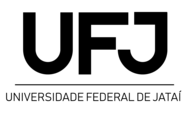
\includegraphics[width=1.5cm]{images/ufjJataiLogo.png}}

\begin{document}

	\begin{frame}
		\titlepage
	\end{frame}

	\AtBeginSection{
		\begin{frame}{Sumário}%[allowframebreaks]{Sumário}
    		\tableofcontents[currentsection]
    		%\tableofcontents[currentsection, hideothersubsections]
		\end{frame}
	}

	\begin{frame}{Plano de Aula}
		\tableofcontents
		%\tableofcontents[hideallsubsections]
	\end{frame}
	
	\section{Instrução pelos Colegas}
	

    \begin{frame}{Pesquisa 003}
		\begin{block}{[P003]}
			Como foi o estudo prévio?
		\end{block}
		\begin{enumerate}[label=(\Alph*)]
			\item Bom
			\item Razoável
			\item Difícil de entender
			\item Não consegui estudar
		\end{enumerate}
	\end{frame}

    \section{Agentes de Busca}
	\begin{frame}{Agentes Reflexivos e Agentes de Planejamento}
    \begin{block}{Agente reflexivo}
        \begin{itemize}
            \item Escolhe a ação com base no estado/percepção atual.
            \item Pode possuir memória ou um modelo do mundo.
            \item \textbf{Não considera as consequências futuras} das ações.
        \end{itemize}
    \end{block}

    \begin{block}{Agente de planejamento}
        \begin{itemize}
            \item Considera ``o que aconteceria se...?''
            \item Usa um \textbf{modelo de como o mundo evolui} após cada ação.
            \item Busca uma \textbf{sequência de ações} que leve ao objetivo.
        \end{itemize}
    \end{block}
\end{frame}

\begin{frame}{Planejamento: olhar para o futuro}
    \begin{block}{Ideia central}
        Planejar é avaliar como o mundo irá evoluir em resposta às ações,
        usando um modelo do mundo.
    \end{block}

    \begin{center}
        \Large
        Estado atual
        $\;\longrightarrow\;$
        \textbf{ações possíveis}
        $\;\longrightarrow\;$\\
        estados futuros
    \end{center}

    \begin{block}{Planejamento}
        \centering
        \textbf{formular um objetivo}
        $\;+\;$
        \textbf{imaginar consequências}
        $\;+\;$
        \textbf{encontrar uma sequência de ações}
    \end{block}
\end{frame}

\begin{frame}{Questão 008}
    \small

    \begin{block}{[Q008]}
        Um agente está em um ambiente no qual, ao perceber um objetivo
        próximo, ele imediatamente escolhe a ação que parece melhor
        naquele momento. Em determinada situação, essa ação faz o agente
        ficar preso em um ciclo, pois existe uma parede que impede seu
        progresso.

        Qual alteração caracteriza melhor um agente de planejamento?
    \end{block}

    \begin{enumerate}[label=(\Alph*)]
        \item Fazer o agente reagir mais rapidamente às percepções atuais.

        \item Fazer o agente armazenar mais percepções passadas,
        sem considerar seus possíveis efeitos futuros.

        \item Fazer o agente utilizar um modelo do mundo para avaliar
        as consequências das ações antes de escolhê-las.

        \item Fazer o agente escolher sempre a ação que o aproxima
        geometricamente do objetivo.
    \end{enumerate}
\end{frame}

\begin{frame}{Formalização de um Problema de Busca}
\begin{block}{Problema de busca}
Para procurar uma solução, o agente precisa representar o problema por meio de:
\end{block}

\begin{itemize}
    \item {\color{blue}\bf Estado inicial}: onde o agente começa.
    \item {\color{blue}\bf Espaço de estados}: configurações possíveis do mundo.
    \item {\color{blue}\bf Função sucessora}: ações possíveis e seus efeitos.
    \item {\color{blue}\bf Teste de objetivo}: verifica se um estado satisfaz o objetivo.
\end{itemize}

\end{frame}

\begin{frame}{Solução de um Problema de Busca}
\begin{block}{Solução}
Uma solução é um {\color{blue}\bf plano}: uma sequência de ações que transforma o estado inicial em um estado que satisfaz o teste de objetivo.
\end{block}\pause

\begin{center}
    Estado inicial
    $\longrightarrow$
    Ação$_1$
    $\longrightarrow$
    Estado
    $\longrightarrow$
    Ação$_2$
    $\longrightarrow$
    \ldots
    $\longrightarrow$
    Objetivo
\end{center}

\end{frame}

{\logo{}
\begin{frame}{Questão 009}
\small
\begin{block}{[Q009]}
Dois agentes recebem o mesmo objetivo: sair da cidade A e chegar à cidade B. O agente 1 representa apenas as cidades e estradas relevantes para encontrar uma rota. O agente 2 utiliza uma representação muito mais detalhada, incluindo diversas características do mundo real que não afetam a possibilidade de viajar entre as cidades. \\Sobre essa situação, é {\bf correto} afirmar que...
\end{block}

\begin{enumerate}[label=(\Alph*)]
    \item O agente 2 necessariamente encontrará uma solução melhor, pois sua representação contém mais informações sobre o mundo real.
    
    \item Os dois agentes necessariamente encontrarão exatamente a mesma solução, pois possuem o mesmo objetivo.
    
    \item O agente 1 não pode encontrar uma solução válida, pois uma representação de busca precisa reproduzir todos os detalhes do mundo real.
    
	 \item O agente 1 pode encontrar uma solução mais facilmente, pois uma abstração adequada elimina detalhes irrelevantes para o problema.
\end{enumerate}

\end{frame}
}

\begin{frame}{Árvore de Busca}
\begin{block}{Ideia central}
A partir do estado inicial, podemos imaginar diferentes sequências de ações e, portanto, diferentes futuros possíveis.
\end{block}

\begin{center}
    \begin{tikzpicture}[level distance=1.1cm,
        level 1/.style={sibling distance=4cm},
        level 2/.style={sibling distance=2cm}]
        \node {Estado inicial}
            child {node {Estado A}
                child {node {Estado C}}
                child {node {Estado D}}}
            child {node {Estado B}
                child {node {Estado C}}
                child {node {Estado E}}};
    \end{tikzpicture}
\end{center}

\end{frame}

\begin{frame}{Estado $\neq$ Nó}
\begin{block}{Estado}
Representa uma configuração do problema.
\end{block}\pause

\begin{block}{Nó da árvore de busca}
    Representa um {\color{blue}\bf estado + o caminho (plano) usado para chegar até ele}.
\end{block}\pause

\begin{center}
    Dois caminhos diferentes podem chegar ao {\color{blue}\bf mesmo estado}.
\end{center}

\end{frame}

\begin{frame}{Questão 010}

\begin{block}{[Q010]}
Durante a expansão, dois caminhos diferentes chegam ao mesmo estado $S$. Qual afirmação está mais adequada sobre a modelagem desse caso?
\end{block}

\begin{enumerate}[label=(\Alph*)]
    \item Na árvore de busca, os dois casos devem ser o mesmo nó, pois estado e nó são equivalentes.
    
    \item Na árvore de busca, são nós diferentes; em busca em grafo, pode haver fusão/pruning com critério sobre caminhos.
    
    \item Se os custos acumulados forem iguais, os nós passam a ser equivalentes em qualquer representação.
    
    \item Dois caminhos distintos nunca devem atingir o mesmo estado em problemas bem formulados.
\end{enumerate}

\end{frame}

\begin{frame}{Fronteira}

\begin{block}{Fronteira (fringe)}
Na busca em árvore, mantemos uma \textbf{fronteira (fringe)} de planos parciais.
Cada expansão remove um nó da fronteira, gera sucessores e adiciona novos planos.
\end{block}

\begin{itemize}
        \item O ponto central é o \textbf{critério de escolha} do próximo nó da fronteira.
        \item \textbf{DFS} (Busca em Profundidade): expande o nó mais profundo.
        \item \textbf{BFS} (Busca em Largura): expande o nó mais raso.
        \item \textbf{UCS} (Busca de Custo Uniforme): \\expande o nó com menor custo acumulado $g(n)$.
        \item Esse critério muda completude, \\otimalidade e custo de tempo/memória.
\end{itemize}
\end{frame}

{\logo{}
\begin{frame}{Questão 011}
\small
\begin{block}{[Q011]}
Considere a fronteira atual com três nós:
\[
\begin{array}{l}
p_1: \text{profundidade } 4,\ g=7 \\
p_2: \text{profundidade } 2,\ g=9 \\
p_3: \text{profundidade } 3,\ g=5
\end{array}
\]

Qual alternativa descreve corretamente o próximo nó expandido por cada estratégia?
\end{block}

\begin{enumerate}[label=(\Alph*)]
        \item DFS, BFS e UCS escolhem $p_3$, pois ele tem menor custo.

        \item DFS escolhe $p_1$; BFS escolhe $p_2$; UCS escolhe $p_3$.

        \item BFS e UCS sempre escolhem o mesmo nó quando os custos são positivos.

        \item DFS e UCS sempre escolhem o mesmo nó quando todos os custos de ação são 1.
\end{enumerate}
\end{frame}
}


% 	\begin{frame}{Agentes Inteligentes}
% 		\begin{block}{Agente}
% 			Um {\color{blue} \bf agente} é tudo o que pode ser considerado capaz de perceber seu {\color{blue} \bf ambiente} por meio de {\color{blue} \bf sensores} e de agir sobre esse ambiente por intermédio de {\color{blue} \bf atuadores}.
% 		\end{block}	
% 	\end{frame}
	
% 	\begin{frame}{Agentes Inteligentes}
% 		\begin{center}
%     		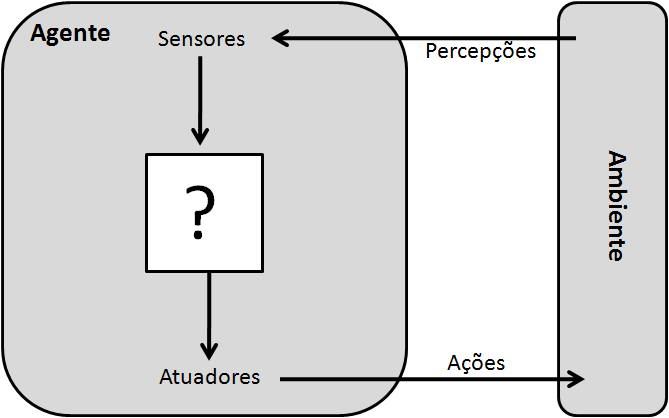
\includegraphics[width=.8\textwidth]{images/esquema.png}
%   		\end{center}
% 	\end{frame}
	
% 	\begin{frame}{Agentes Inteligentes}
% 		\begin{block}{Agente}
% 			Um {\color{blue} \bf agente} é tudo o que pode ser considerado capaz de perceber seu {\color{blue} \bf ambiente} por meio de {\color{blue} \bf sensores} e de agir sobre esse ambiente por intermédio de {\color{blue} \bf atuadores}.
% 		\end{block}
% 		\begin{block}{Percepção}
% 			\begin{itemize}						
% 				\item O termo {\color{blue} \bf percepção} é uma referência às entradas perceptivas do agente em qualquer momento dado;
% 				\item Uma {\color{blue} \bf sequência de percepções} do agente é a história completa de tudo o que o agente já percebeu.
% 			\end{itemize}
% 		\end{block}
% 	\end{frame}
	
% 	\begin{frame}{Mundo do Aspirador de Pó}
% 		\begin{center}
%     		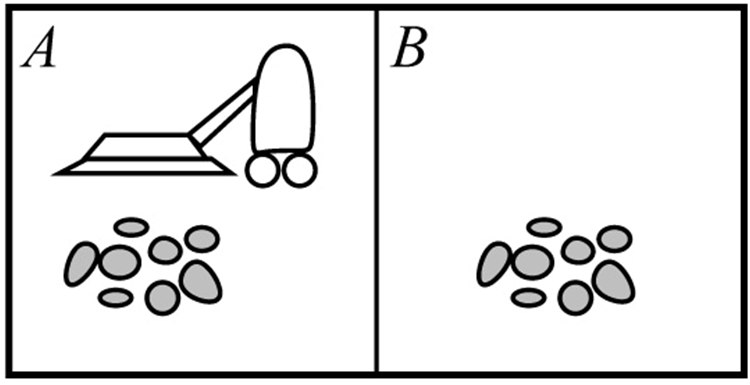
\includegraphics[width=.8\textwidth]{images/aspirador.png}
%   		\end{center}
% 	\end{frame}
    
%     \begin{frame}{Agentes Inteligentes}
% 		\begin{block}{Função de agente}
% 			É uma {\color{blue} \bf função} que descreve o comportamento do agente mapeando qualquer sequência de percepções específica para uma ação. 
% 		\end{block}	\pause
% 		\begin{block}{Programa de agente}
% 			\begin{itemize}						
% 				\item É uma {\color{blue} \bf implementação concreta} da descrição matemática abstrata da função de agente. Esta implementação {\color{blue} \bf depende da arquitetura} do agente.
% 			\end{itemize}
% 		\end{block}
% 	\end{frame}
	
% 	\begin{frame}{Mundo do Aspirador de Pó}
% 		\begin{center}
%     		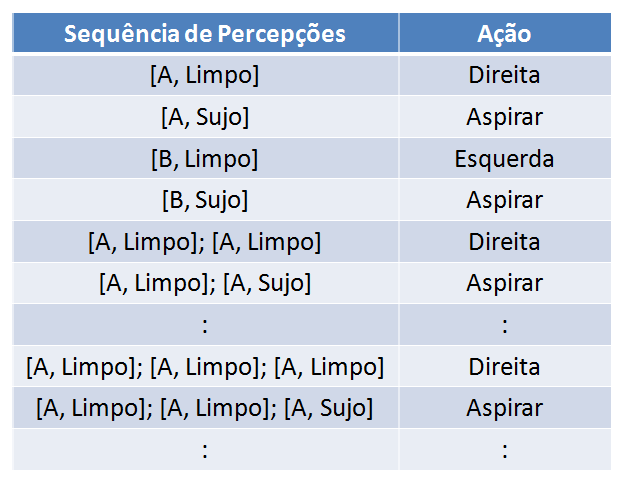
\includegraphics[width=.8\textwidth]{images/tabela.png}
%   		\end{center}
% 	\end{frame}

% 	\begin{frame}{Questão 005} 
% 		\footnotesize
% 		\begin{block}{[Q005]} 
% 			Considere dois agentes que atuam no mesmo ambiente e recebem exatamente as mesmas percepções. O agente A implementa uma determinada função de agente por meio de uma tabela, enquanto o agente B implementa a mesma função por meio de um programa baseado em regras. Sobre essa situação, é correto afirmar que... 
% 		\end{block} 
% 		\begin{enumerate}[label=(\Alph*)] 
% 			\item A e B necessariamente produzem comportamentos diferentes, pois utilizam programas diferentes. 
% 			\item A e B podem produzir exatamente o mesmo comportamento, pois programas diferentes podem implementar a mesma função de agente. 
% 			\item A implementa uma função de agente, enquanto B implementa um programa de agente; portanto, apenas B possui comportamento definido. 
% 			\item A função de agente e o programa de agente são conceitos equivalentes, pois ambos recebem a percepção atual e retornam uma ação. 
% 		\end{enumerate} 
% 	\end{frame}


%         \begin{frame}{Medida de Desempenho}
% 		\begin{block}{Medida de Desempenho}
% 			É um {\color{blue} \bf critério} para se medir o sucesso do agente.
% 		\end{block}	\pause
% 		\begin{block}{A racionalidade depende...}
% 			\begin{itemize}						
% 				\item Da {\color{blue} \bf medida de desempenho};
%  				\item Do conhecimento anterior do agente sobre o {\color{blue} \bf ambiente};
%  				\item Das {\color{blue} \bf ações} que o agente pode executar;
%  				\item Da sequência de {\color{blue} \bf percepções} do agente até o momento.
% 			\end{itemize}
% 		\end{block}
% 	\end{frame}
	
% 	\begin{frame}{Logo a racionalidade é...}
% 		\begin{block}{}
% 			``Para cada {\color{blue} \bf sequência de percepções} possível, um agente racional deve selecionar uma {\color{blue} \bf ação} que venha maximizar sua {\color{blue} \bf medida de desempenho}, dada a evidência fornecida pela sequência de percepções e por qualquer {\color{blue} \bf conhecimento interno} do agente''.
% 		\end{block}
% 	\end{frame}

% 	\begin{frame}{Questão 006}
% 		\footnotesize

%     \begin{block}{[Q006]}
%         Um agente aspirador de pó foi projetado para:

%         \begin{itemize}
%             \item receber 1 ponto a cada instante em que um quadrado está limpo;
%             \item pagar uma penalidade de 1 ponto sempre que se mover.
%         \end{itemize}

%         Depois que os dois quadrados já estão limpos, o agente continua
%         alternando entre eles.

%         Considerando essa nova medida de desempenho, qual avaliação
%         é mais adequada?
%     \end{block}

%     \begin{enumerate}[label=(\Alph*)]

%         \item O agente continua necessariamente racional, pois sua função
%         de agente não mudou.

%         \item O agente pode ter se tornado irracional, pois a racionalidade
%         depende também da medida de desempenho adotada.

%         \item O agente é irracional porque um agente racional nunca deve
%         executar a mesma ação mais de uma vez.

%         \item O agente continua racional, pois realizar mais ações sempre
%         aumenta a experiência do agente.

%     \end{enumerate}

% \end{frame}
	
% 	\begin{frame}{Onisciência {\it versus} Racionalidade}
% 		\begin{block}{Onisciência}
% 			Um agente onisciente sabe o {\color{blue} \bf resultado real} de suas ações e pode agir de acordo em relação a ele.
% 		\end{block}	\pause
% 		\begin{block}{Racionalidade}
% 			Um agente racional sabe o {\color{blue} \bf resultado esperado} de suas ações e pode agir de acordo em relação a ele.
% 		\end{block}
% 	\end{frame}

% 	\begin{frame}{Questão 007}

% 		\small

%     \begin{block}{[Q007]}
%         Um agente precisa atravessar uma rua. Seus sensores ainda não
%         permitem determinar se há veículos se aproximando.

%         Um estudante afirma:

%         \begin{quote}
%         ``Como o agente não sabe o que acontecerá, qualquer ação que ele
%         escolher será igualmente racional.''
%         \end{quote}

%         Qual resposta melhor explica por que essa afirmação está incorreta?
%     \end{block}

%     \begin{enumerate}[label=(\Alph*)]

%         \item Um agente racional deve sempre escolher a ação que produz
%         o melhor resultado real.

%         \item Um agente racional não pode agir em ambientes parcialmente
%         observáveis.

%         \item O agente deve considerar que ações (como obter mais informação) podem aumentar seu desempenho esperado antes da decisão.

%         \item Se o resultado não puder ser conhecido com certeza, a única
%         escolha racional é não fazer nada.

%     \end{enumerate}

% \end{frame}

	
	
	\begin{frame}
		\titlepage
	\end{frame}
	
\end{document}